\documentclass{article}
\usepackage{graphicx}
\usepackage{float}
\usepackage[margin=1in]{geometry} 
\usepackage{amsmath,amsthm,amssymb,hyperref}
\usepackage{caption}
\usepackage{subcaption}

\newcommand{\R}{\mathbf{R}}  
\newcommand{\Z}{\mathbf{Z}}
\newcommand{\N}{\mathbf{N}}
\newcommand{\Q}{\mathbf{Q}}

\newenvironment{theorem}[2][Theorem]{\begin{trivlist}
\item[\hskip \labelsep {\bfseries #1}\hskip \labelsep {\bfseries #2.}]}{\end{trivlist}}
\newenvironment{lemma}[2][Lemma]{\begin{trivlist}
\item[\hskip \labelsep {\bfseries #1}\hskip \labelsep {\bfseries #2.}]}{\end{trivlist}}
\newenvironment{exercise}[2][Exercise]{\begin{trivlist}
\item[\hskip \labelsep {\bfseries #1}\hskip \labelsep {\bfseries #2.}]}{\end{trivlist}}
\newenvironment{problem}[2][Problem]{\begin{trivlist}
\item[\hskip \labelsep {\bfseries #1}\hskip \labelsep {\bfseries #2.}]}{\end{trivlist}}
\newenvironment{question}[2][Question]{\begin{trivlist}
\item[\hskip \labelsep {\bfseries #1}\hskip \labelsep {\bfseries #2.}]}{\end{trivlist}}
\newenvironment{corollary}[2][Corollary]{\begin{trivlist}
\item[\hskip \labelsep {\bfseries #1}\hskip \labelsep {\bfseries #2.}]}{\end{trivlist}}

\newenvironment{solution}{\begin{proof}[Solution]}{\end{proof}}

\begin{document}


\title{Spruce Budworm Outbreak}
\author{Varenya Upadhyaya EP20BTECH11026} 
\date{}
\maketitle

\section{Introduction}
Spruce Budworms are moths native to North America (more specifically, East USA and Canada). They generally feed on the Balsam Fir and White Spruce trees. Their population often experiences significant oscillations with large outbreaks that result in massive scale defoliation of Canadian forests. The first recorded outbreak was in 1807 and since the 1900s these outbreaks have been happening in around every forty years. The drastic effect of these pests on the ecosystem call for some study on the frequency of these outbreaks along with a quantitative analysis of the impact they have on trees.\\
In our analysis, we will be using a model proposed by \href{https://www.jstor.org/stable/3939?seq=1}{D. Ludwig, D. D. Jones and C.S. Holling}.\\

\section{Applying the NLD Model}
In their paper they proposed the following model:
\begin{align}
    \dot{N} = RN(1-\frac{N}{K}) - p(N) \label{eq1}
\end{align}
where $N(t)$ represents the Budworm population, $R$ and $K$ represent the Growth rate of the budworms and Carrying capacity of the forest. $p(N)$ is the predation term which accounts for the worms being eaten by birds (the predators).
% \subsection{The predation function}
The following function is used for predation
\begin{align}
    p(N) = \frac{N^2}{1+N^2}
\end{align}
The above formula for $p(N)$ contains no parameters to adjust the rate at which the worms are eaten as the population increases. This alters the interpretation of $R$, $K$ and $N$. For instance, $N=n$ indicates the budworm population where the birds are eating at $n^2/{1+n^2}$ of their maximum rate.
Fig. \ref{fig:pred} shows the plot of the predation function. 
\begin{figure}[H]
    \centering
        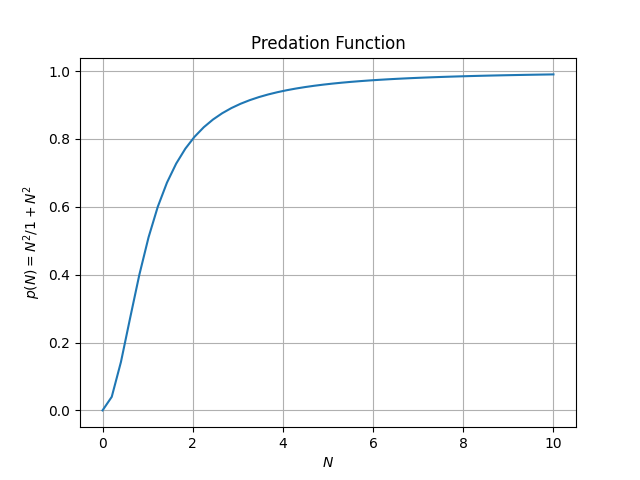
\includegraphics[width=8cm]{PredationFigure.png}
    \caption{$p(N)$}
    \label{fig:pred}
\end{figure}
Changing the variables (as per convention), we can thus write Eq.\eqref{eq1} as:
\begin{align}
        \dot{x} = rx(1-\frac{x}{k}) -\frac{x^2}{1+x^2}
\end{align}
where $r$ and $k$ are now dimensionless growth rate and carrying capacity respectively.\\
With the model ready, we can now analyze the situations leading up to the outbreak, the outbreak and the eventual decline.\\

\section{Before the outbreak: The Build-up}
For starters, we consider the situation when $r=0.52$ and $k=3.6$. As seen in the figure \ref{fig:b1}, we find two equilibrium points, one at $x=0$ and another at $x=0.58$. Clearly the first one is an unstable equilibrium whereas the second one is stable. The value for $k$ is relatively small for now, corresponding to a tiny forest. Consider the predation function for the stable equilibrium state in this situation:
\begin{align}
    p(x) &= \frac{x^2}{1+x^2},\hspace{10pt} x=0.58\\
    \implies p(0.58) &= 0.25
\end{align}
Seeing how the function can reach a maximum value of 1, we can conclude that the birds are consuming the worms at $25\%$ of their capacity (keeping the worms in check).
As the value of $k$ goes up to 7.5 (Fig. \ref{fig:b2}), we can see that now there are 4 equilibrium states:
\begin{align*}
    x&=0\\
    x&=0.70\\
    x&=2.44\\
    x&=4.35
\end{align*}
,out of which the second and fourth are stable ones. The lower equilibrium is quite close to what we saw previously however there is now an upper one to consider $x=4.35$.
The predating function at this equilibrium will be:
\begin{align}
    p(x) &= \frac{x^2}{1+x^2},\hspace{10pt} x=4.35\\
    \implies p(4.35) &= 0.95
\end{align}
implying that the predators have nearly reached their maximum capacity.

This shows that if we started with a small forest (with a small budworm population) that grew to around $k=7.5$, the population would converge to the second equilibrium (corresponding to the outbreak) for all $x>2.44$. If we now increase $k$ all the way to 20 9\ref{fig:b3}, no qualitative change takes place but the last stable equilibrium gets shifted to $x=17.85$. As the forest grows, the spruce budworm population also increases and the predators fail to keep it in check.
\begin{figure}[H]
     \centering
     \begin{subfigure}[b]{0.3\textwidth}
         \centering
         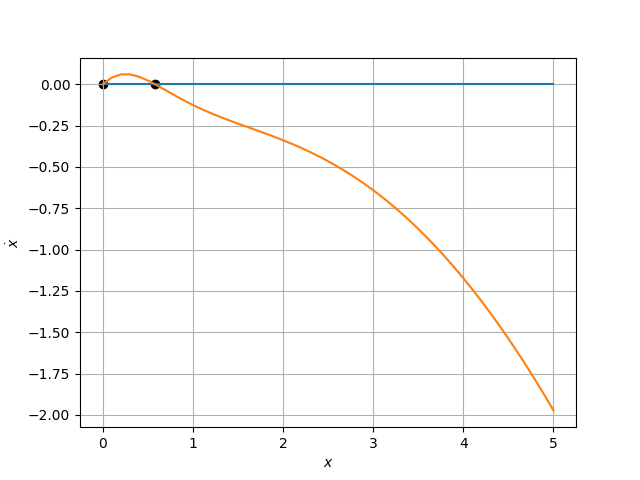
\includegraphics[width=\textwidth]{buildup1.png}
         \caption{$k=3.6$}
         \label{fig:b1}
     \end{subfigure}
     \hfill
     \begin{subfigure}[b]{0.3\textwidth}
         \centering
         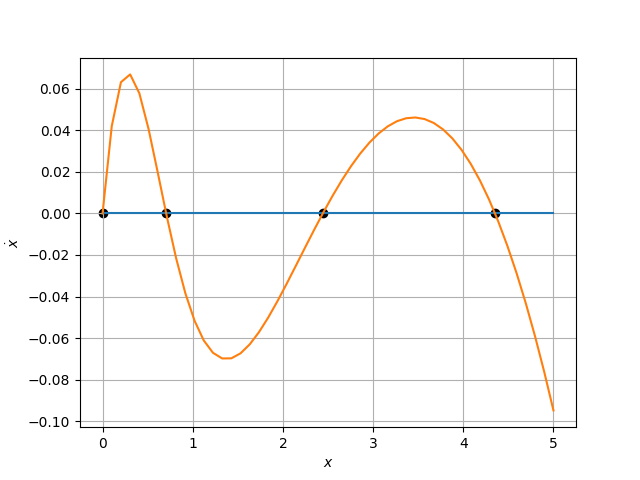
\includegraphics[width=\textwidth]{buildup2.png}
         \caption{$k=7.5$}
         \label{fig:b2}
     \end{subfigure}
     \hfill
          \begin{subfigure}[b]{0.3\textwidth}
         \centering
         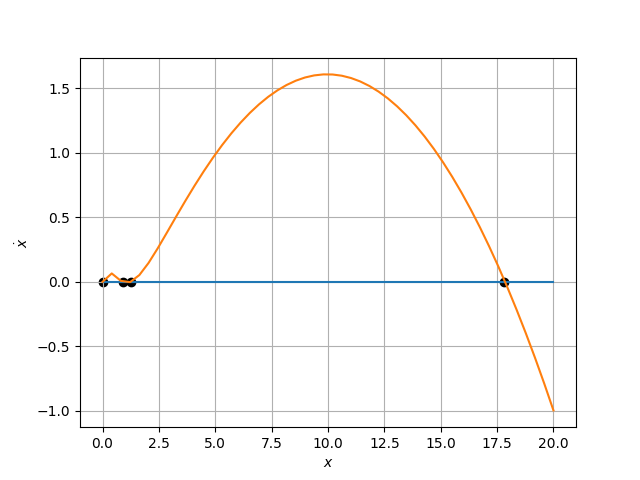
\includegraphics[width=\textwidth]{buildup3.png}
         \caption{$k=20$}
         \label{fig:b3}
     \end{subfigure}
        \caption{$\dot{x}$ for various values of $k$ at $r=0.52$}
        \label{fig:buildup}
\end{figure}
\section{The Outbreak}
Now, we consider the case where the forest grows to $k=27$. We encounter a saddle-node bifurcation with the fixed points coalescing into a single half stable fixed point at $x=1.04$. As the forest continues to grow to $k=30$, we're left with only one fixed point at $x=27.94$, corresponding to the outbreak. The predation factor at this stage:
\begin{align}
    p(x) &= \frac{x^2}{1+x^2},\hspace{10pt} x=27.94\\
    \implies p(27.94) &= 0.9987 \approx 1
\end{align}
The birds are eating the worms at their maximum capacity, however this isn't enough to keep the worm population in check. A $k$ goes up to 30, we get $x\approx30$, which means that there are budworms, eating leaves off trees throughout the forest.
Fig. \ref{fig:o1} and Fig. \ref{fig:o2} depict the state of the forest during the outbreak.
\begin{figure}[H]
     \centering
     \begin{subfigure}[b]{0.4\textwidth}
         \centering
         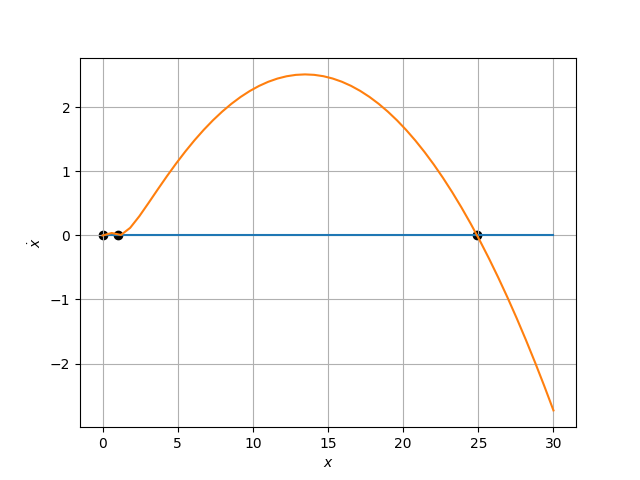
\includegraphics[width=\textwidth]{outbreak1.png}
         \caption{$k=27$}
         \label{fig:o1}
     \end{subfigure}
    %  \hfill
     \begin{subfigure}[b]{0.4\textwidth}
         \centering
         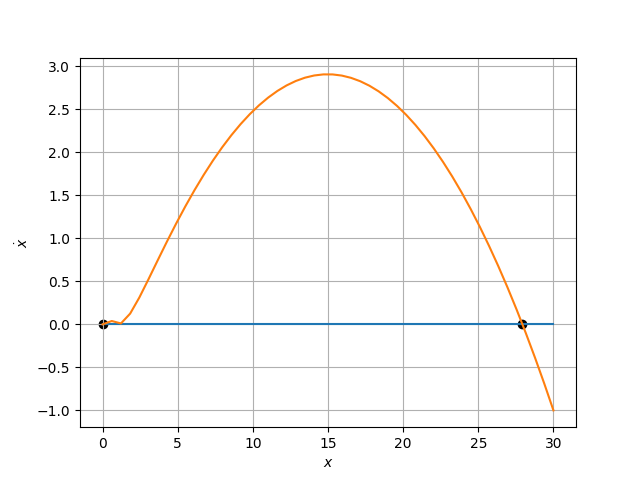
\includegraphics[width=\textwidth]{outbreak2.png}
         \caption{$k=30$}
         \label{fig:o2}
     \end{subfigure}
             \caption{$\dot{x}$ during the Outbreak}
        \label{fig:outbreak}
\end{figure}
\section{After the outbreak: The Decline}
After a prolonged outbreak, the pests cause a vast defoliation of the trees in the forest, thereby decreasing the amount of food available to them. Due to a lack of food, most of the worms will die of starvation. We now analyse how the model factors in case of the decline.\\
As the forest is dying, the carrying capacity $k$ starts reducing again. At $k=20$ the system is still in a stable equilibrium corresponding to the outbreak. However this just means that the carrying capacity will keep decreasing with a large budworm population around. We will consider two main cases here, first at $k=7.5$ and then $k=6.5$.\\
When $k=7.5$ (Fig. \ref{fig:d1}, as we had above, the function has 4 fixed points out of which two are stable. Owing to the large population, $x$ will shrink to reach the equilibrium at $x=4.35$ while constantly reducing the carrying capacity of the forest.\\
A drastic change occurs when $k$ drops to 6.5 (Fig. \ref{fig:d2}, the latter two fixed points coalesce, eventually leaving only two equilibrium points: $x=\{0, 0.682\}$. The budworm population will thus converge to $x=0.682$, leading to an overall decline in the outbreak. Another factor which aids the decline is the predation. The birds continue to eat the worms that don't die due to starvation, thereby nearly wiping out the entire Spruce Budworm population.


\begin{figure}[H]
     \centering
     \begin{subfigure}[b]{0.4\textwidth}
         \centering
         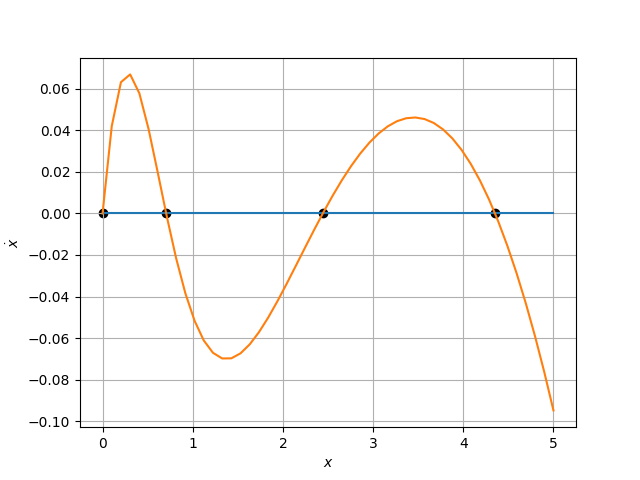
\includegraphics[width=\textwidth]{buildup2.png}
         \caption{$k=7.5$}
         \label{fig:d1}
     \end{subfigure}
    %  \hfill
     \begin{subfigure}[b]{0.4\textwidth}
         \centering
         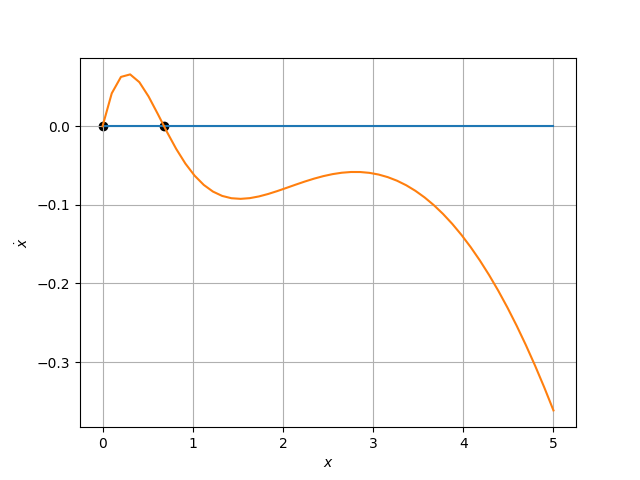
\includegraphics[width=\textwidth]{decline1.png}
         \caption{$k=6.5$}
         \label{fig:d2}
     \end{subfigure}
             \caption{$\dot{x}$ During the Decline}
        \label{fig:decline}
\end{figure}

\section{Summary and Conclusions}
To summarise, we plot a bifurcation curve with $x$ on the vertical axis and $k$ on the horizontal axis. Fig. \ref{fig:s1} and Fig. \ref{fig:s2}, show how the budworm population $x(t)$ changes with the carrying capacity.
 \begin{figure}[H]
     \centering
     \begin{subfigure}[b]{0.4\textwidth}
         \centering
         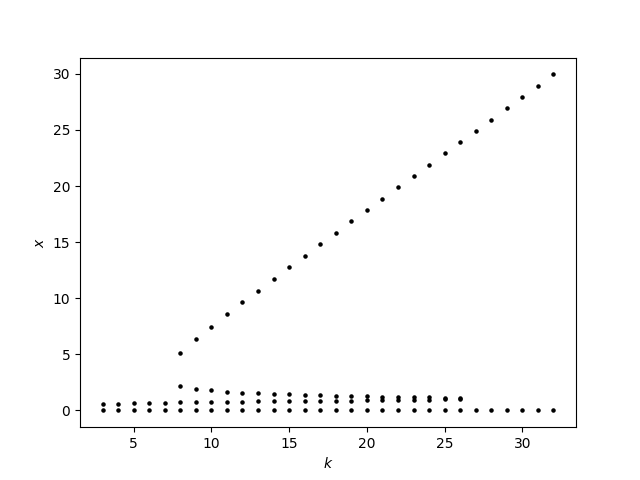
\includegraphics[width=\textwidth]{summary1.png}
         \caption{Scatter plot of the equilibrium\\ points for different $k$}
         \label{fig:s1}
     \end{subfigure}
    %  \hfill
     \begin{subfigure}[b]{0.4\textwidth}
         \centering
         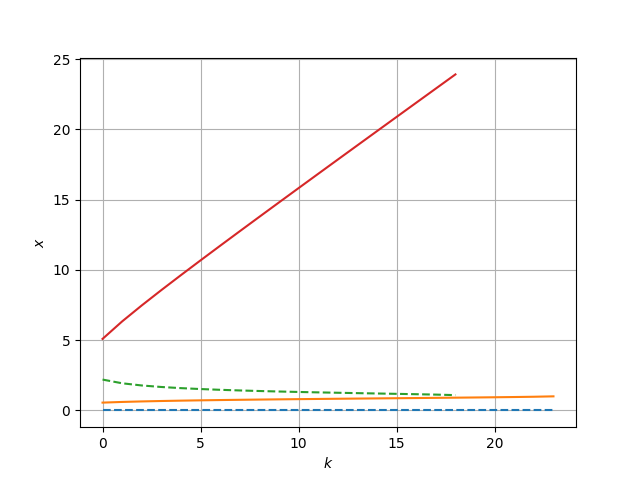
\includegraphics[width=\textwidth]{summary2.png}
         \caption{A continuous plot with solid/dashed lines\\ representing stable/unstable states }
         \label{fig:s2}
     \end{subfigure}
             \caption{Bifurcation Plots}
        \label{fig:summary}
        \end{figure}
Thus, when we start with a small budworm population in a small forest with predators, the population increases rapidly and then eventually starts declining due to various factors (starvation and predators). This cycle tends to repeat itself around every 40 years in the Canadian forests.
\section{References}
\begin{itemize}
    \item Nonlinear Dynamics and Chaos: Strogatz, S. H.
    \item \url{https://www.nrcan.gc.ca/our-natural-resources/forests/wildland-fires-insects-disturbances/top-forest-insects-and-diseases-canada/spruce-budworm/13383}
    \item \url{https://mathinsight.org/spruce_budworm_outbreak_model}
\end{itemize}
The figures and python code (for the figures) can be found at: \url{https://github.com/varenya27/NLD-Project}
\end{document}